%!TEX root = ../main.tex

\section{Evaluation} % (fold)
\label{sec:evaluation}

The evaluation will be divided into three separate test scenarios. 
As we are looking into how we can convey weather data through sonification, and how intuitively understood this information compared to visual representations of similar data is. 
It will be possible to evaluate upon by isolating and comparing data from several tests, where one test is of the produced sonifications, another test with visual elements and one test where both visuals and sonifications is tested.


More specifically described, a test will be conducted solely where the weather sonifications are presented to test subjects.
Similar, a test will be conducted where the visual representations will be presented with the same procedure as the sonification, and finally a test where both visual representations along with the sonification of the data.
This procedure will make it possible to compare what the test subjects can deduct from the presented data, and allow us to make comparisons towards what information the visual, sonification and combined representations of data is conveying, and thereby make it possible to evaluate upon how well the sonification formulate weather data.


\subsection{Method} % (fold)
\label{sub:method}

The primary reason of the evaluation is to establish knowledge as to determine if the list of requirements has been fulfilled and to make it possible to gain satisfying results which helps answering the final problem statement.


The implemented product contains sonifications of specific weather categories, where these categories has been further categorised into sonifications of different values which represent low, medium and high values of a specific weather category.

A Kruskal-Wallis test will be conducted on the gathered test results, which will be separated into three separate tests. 
This will ensure that it is possible to distinguish between the results gathered from the low values, medium values and the high values of the weather data, and will provide 3 seperate box plots and associated data, which will allow us to prove or disprove the null hypothesis and to make assumptions and further analysis which will help answering the final problem statement.


\subsection{Procedure} % (fold)
\label{sub:procedure}

Here are the procedure for the test explained in detail. This chapter will describe the different aspects of the test such as sampling, observations, and guidelines for the testing. The same test procedure will be done on three separate presentations of weather conditions: visual presentation, audial representation, and combined presentation.
The general data for the tests are presented below.


Amount of participants: 20 subjects per category per presentation.
Test subject sampling: Convenience sampling: Aalborg university students.
Estimated length of test: 1 minute per subject.
Test location: Area on and around Aalborg university.
Date and time: When appropriate.


\subsubsection{Test setup} % (fold)
\label{ssub:test_setup}

The test will not require any specific location. 
For the testing only two people are present, i.e. 1 test subject and the test conductor. 
Only the combined test required two conductors for convenience purposes. The test subject and observer will be placed opposite each other during the test.
Other individuals, in this case other test subjects, will be placed out of view to avoid bias by previous subjects answers.

% subsubsection test_setup (end)


\subsubsection{Test Materials} % (fold)
\label{ssub:test_materials}

\subsubsection*{Visual test} % (fold)
\label{ssub:visual_test}

\begin{itemize}
    \item Visual samples: A set of images each representing a separate weather condition. The samples will be be presented to the subject one at a time to avoid that the subject makes assumptions based on the other samples.
    \item  Notation sheets: Sheets of paper where the presented samples and respective responses are recorded.
\end{itemize}

% subsubsection visual_test (end)


\subsubsection*{Sound test} % (fold)
\label{ssub:sound_test}

\begin{itemize}
    \item Audio samples: A set of audio snippets each representing a separate weather condition. The samples will be produced on scene using Pure Data and will not be prerecorded.
    \item Notation sheets: Sheets of paper where the presented samples and respective responses are recorded.
\end{itemize}

% subsubsection sound_test (end)

\subsubsection*{Combined test} % (fold)
\label{ssub:combined_test}

\begin{itemize}
    \item Visual samples: The same samples from the visual test.
    \item Audio samples: the same samples from the audial test.
    \item Notation sheets.
\end{itemize}

% subsubsection combined_test (end)

% subsubsection test_materials (end)


\subsubsection{Test Execution} % (fold)
\label{ssub:test_execution}

The testing procedure differs slightly in the three tests. 
In the visual test the subject is presented an image of a weather condition. 
The images does not contain the actual weather data they try to represent. 
During the audio test the subject is presented with an audio sample produced by Pure Data, and in the combined test the subject is presented with both an image and an audio sample of the same weather condition.


The overall testing execution looks like this:

\begin{itemize}
    \item The subject is placed opposite the observer.
    \item The observer presents the subject with a sample. The samples does not have to be in any kind of order because the subject has no knowledge of the different weather conditions that will be presented.
    \item The presented sample is noted by the observer and the observer ask the subject if the if the sample presents a low, medium, or high value.
    \item The observer notes the answer and continues to the next sample until a sample from each category has been answered.
\end{itemize}

Before each test the subjects are informed that they are to be presented with 5 different samples (one for each category).
They will be asked a question to each sample and that they are only to answer "high", "medium", or "low" to the questions. 
In order to ensure that each subject has the same understanding of the samples they are given some context for each sample.
This is done through the question asked to each sample. 
The question contains the weather condition but not the actual data i.e. "How much wind is in this image, high, medium, or low?". 
The subject will not be given any further clarification as we are looking for the intuitive guess and not the qualified guess.

% subsubsection test_execution (end)


\subsection{Hypothesis} % (fold)
\label{sub:hypothesis}

Based upon the formulation of the final problem statement, the scientific experiment can be deducted into two separate hypotheses. 
One hypothesis which specifies that there are no significant difference between the samples, and one hypothesis which specifies that there is some significant difference.


\subsubsection{Null Hypothesis} % (fold)
\label{ssub:null_hypothesis}

There is no significant difference between the understanding of the non-speech auditory display of weather data using sonification techniques, compared to the understanding of visually presented weather information.

% subsubsection null_hypothesis (end)


\subsubsection{Alternative Hypothesis} % (fold)
\label{ssub:alternative_hypothesis}

There is some significant difference between the understanding of the non-speech auditory display of weather data using sonification techniques, compared to the understanding of visually presented weather information.

% subsubsection alternative_hypothesis (end)

\subsubsection{Test Delimitation} % (fold)
\label{ssub:test_delimitation}

In order to prove or disprove the Null hypothesis, a statistical test is specified.
The method of establishing knowledge towards what test will be used, the structure from Andy Field \& Graham Hole is utilized \cite[c.8][]{Field2003}.

\subsubsection{Type of data that is collected} % (fold)
\label{ssub:type_of_data_that_is_collected}

The data that is collected from the test participants is considered scores. 
As we are collecting data through a scientific study, the data that is contributed from the test participants are nominal data, being data that uses numbers to define categories or range of values which the test subjects think is correct.


What is obtained from the test participants is a value from 1-3 indicating low, medium or high values of a specific weather condition, which indicates their intuitive thought of what the formulated weather data represents.

% subsubsection type_of_data_that_is_collected (end)

\subsubsection{Independent variables} % (fold)
\label{ssub:independent_variables}

Independent variables, being something that is manipulated by us, is the weather conditions. 
There are one independent variable in this study, being the specific formulation of a single weather condition. 
As an example, the test subjects are presented with low/little rain as a visual image. 
Other test subjects are also presented with low/little rain, but as a sonification, or both. 
Then the test subjects provide scores, indicating what they actually think is presented.

% subsubsection independent_variables (end)

\subsubsection{Experiment design} % (fold)
\label{ssub:experiment_design}

As we are looking for differences or similarities between groups of which we have altered independent variables, an experimental design is utilized.

% subsubsection experiment_design (end)

\subsubsection{Independent measures} % (fold)
\label{ssub:independent_measures}

Since we look for intuitively understanding of a sonification of weather data, each participant will only be subjected to one condition of the test. 
This will allow us to obtain a single score from each participant in either the sonification, visual, or sonification \& visual test. 
The study can therefore be described as a wholly independent measure design test.


The test subjects will be allowed to contribute with several answers within the same condition, but will not be allowed to contribute to others.

% subsubsection independent_measures (end)

\subsubsection{Non-parametric} % (fold)
\label{ssub:non_parametric}

As we have no pre-defined assumptions to the test, and to what extent there might be certain characteristics, the study can be described as non-parametric.

% subsubsection non_parametric (end)

\subsubsection{Test groups} % (fold)
\label{ssub:test_groups}

As specified as the independent variable, there are three different groups which contributed with scores.

% subsubsection test_groups (end)

\subsubsection{Kruskal-Wallis Test} % (fold)
\label{ssub:kruskal_wallis_test}

By delimitating the above mentioned steps, it is defined that a Kruskal-Wallis test can be utilized to prove or disprove the Null hypothesis.


A Kruskal-Wallis test compares between the medians of two or more samples, to determine if the samples have come from different populations \cite*{Gaten2000}.


There are however, the following limitations to the Kruskal-Wallis test.
If no significant difference in our data is found, the samples can not be concluded as to being similar.
If there are any significant difference, it is not possible to make specific assumptions as towards what contributed to the significant difference. 
Further analysis and testing would be required \cite*{Gaten2000}.
% subsubsection kruskal_wallis_test (end)

% subsubsection test_delimitation (end)

% subsection hypothesis (end)

% subsection procedure (end)

% subsection method (end)

\subsection{Results} % (fold)
\label{sub:results}

The results from the test are here presented and described. 
Discussions and interpretations of the results are conducted in the Evaluation: Discussion (See next section XX)

The gathered results can be found in appendix (XX).

\begin{figure}[!htbp]
    \centering
    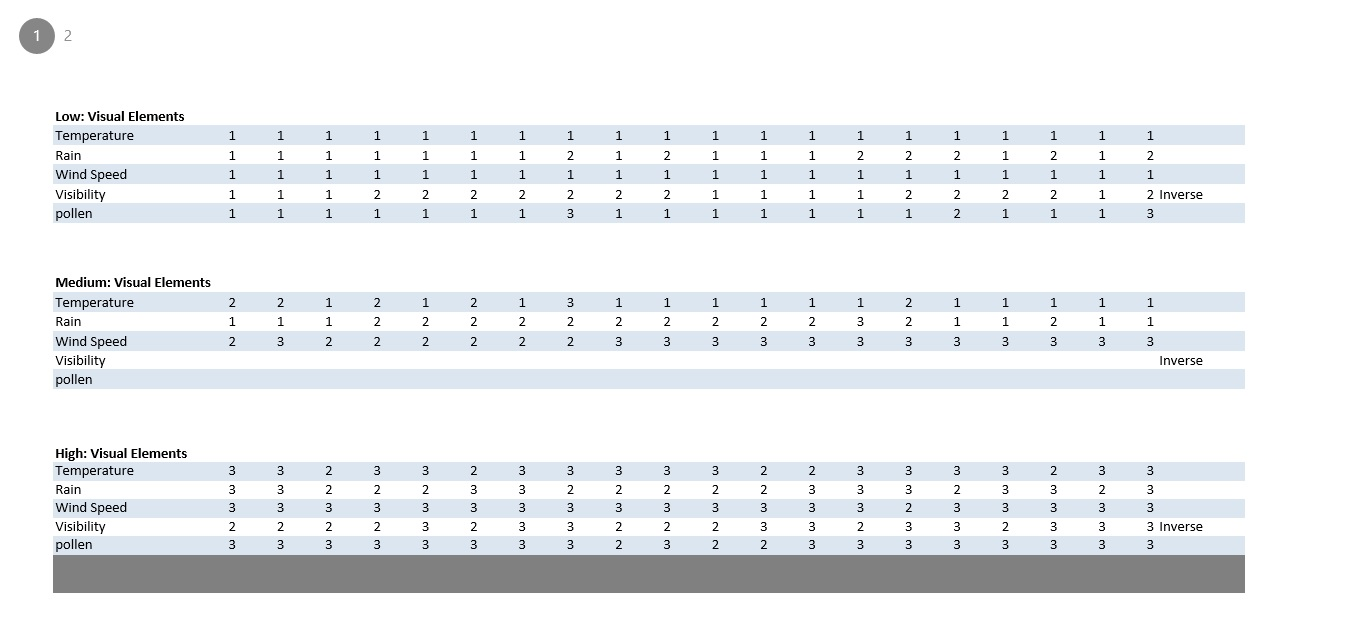
\includegraphics[width=1\textwidth]{images/Evaluation1.jpg}
    \caption{Test result snippet}
    \label{fig:evaluation1}
\end{figure}

As seen on figure~\ref{fig:evaluation1}, there are three categories. 
Low elements, medium elements, and high elements. 
This example only covers the visual weather data. 
The results gathered from Sonification, and sonification \& Visual elements can be found in the appendix(XX).


The numbers indicates the responses from 20 test participants. 
These are labels of 1-2-3 which indicates low, medium and high values.

The rows indicates responses from a single test participant.

\begin{itemize}
    \item Low values has the label: 1
    \item Medium values has the label: 2
    \item High values has the label: 3
\end{itemize}

It can be deducted from the figure, that if a low weather condition which has been answered and labeled with 1, then the answer is correct, as the image illustrates a weather condition of low value. 
Likewise with medium values which has the answer of 2 and high values with the answer of 3. 
If a medium sound is heard, and the test subject answers correctly with a response of medium, then 2 is noted.

\subsubsection{Kruskal-Wallis Test Results} % (fold)
\label{ssub:kruskal_wallis_test_results}

The test results will be divided into three separate Kruskal-Wallis tests, in order to evaluate upon low data, medium data and high data separately, to make the distinction between the independent variable more easily. 
What will be the outcome is a Boxplot, respectively of low, medium and high weather data elements along with the data descriptions of the three Kruskal-Wallis tests. 


\subsubsection*{Low values: Kruskal-Wallis ANOVA table} % (fold)
\label{ssub:low_values_kruskal_wallis_anova_table}

\begin{figure}[!htbp]
    \centering
    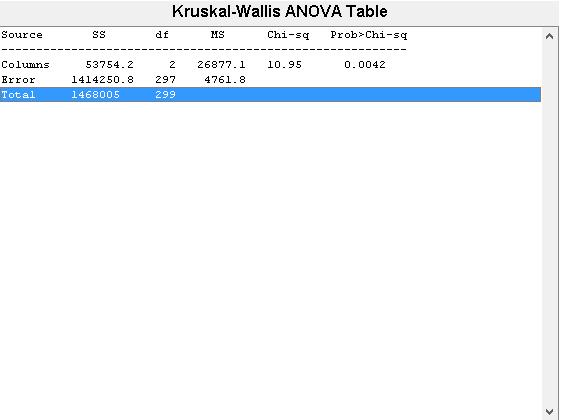
\includegraphics[width=.7\textwidth]{images/Evaluation2.jpg}
    \caption{ANOVA table low data}
    \label{fig:evaluation2}
\end{figure}

The P value(Prob>Chi-sq) is 0.0042 which is under 0.05. Therefore the null hypothesis is rejected and accept the alternative hypothesis.

% subsubsection low_values_kruskal_wallis_anova_table (end)

\subsubsection*{Low values: Kruskal-Wallis test results} % (fold)
\label{ssub:low_values_kruskal_wallis_test_results}

\begin{figure}[!htbp]
    \centering
    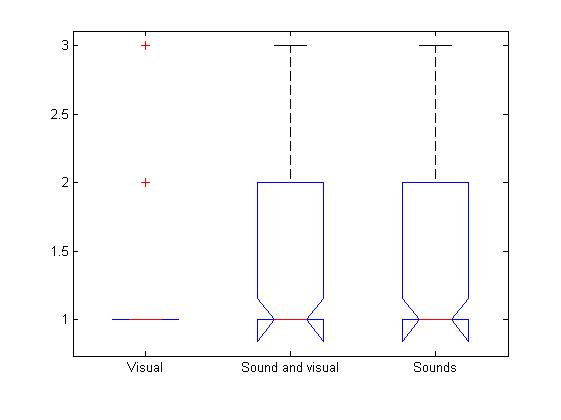
\includegraphics[width=.5\textwidth]{images/Evaluation3.jpg}
    \caption{Boxplot low data}
    \label{fig:evaluation3}
\end{figure}

Generally the boxplot indicates similar levels of medians but the visual scale has a different distribution than "Sound and Visual" and "Sounds".

The "Visual" element is comparatively short, as the inner quartile range is overlapping which suggests that a high number of responses are 1. 
A majority of participants answered correctly, but a low number of participants, indicated by the "plus", that 2 and 3 was also answered by a lower population of the test participants.

% subsubsection low_values_kruskal_wallis_test_results (end)

% subsubsection kruskal_wallis_test_results (end)


\subsubsection{Graphical test results} % (fold)
\label{ssub:graphical_test_results}

As the Kruskal-Wallis test only provides knowledge of statistical differences of the data groups, it is also important to gain knowledge of the specific weather condition elements which proved to be successful or unsuccessful. 
In order to elaborate upon what sounds, compared to the visual elements had any/if any specific impact. 
Therefore a graphical structure of the results are developed. (Appendix XX)

\begin{figure}[!htbp]
    \centering
    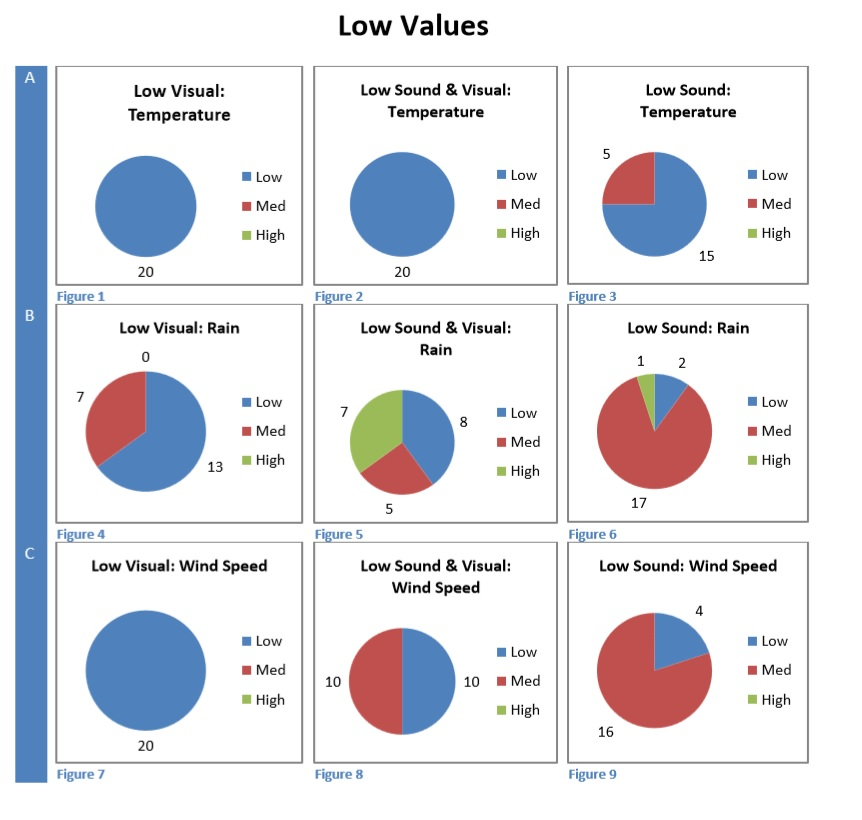
\includegraphics[width=.7\textwidth]{images/Evaluation4.jpg}
    \caption{Snippet of graphic chart: Test Results}
    \label{fig:evaluation4}
\end{figure}

As seen on figure~\ref{fig:evaluation4}, a snippet of the pie charts are presented. 
On the row A1-3, the three temperature results is comparable. 
The pie charts each represents 20 responses and indicates the participants answers of the visual elements, sound and visual elements and the sound element. 
See(Appendix XX. ) for the combined graphical results.

% subsubsection graphical_test_results (end)

% subsection results (end)


\subsection{Discussion} % (fold)
\label{sub:discussion}

Here, the discussion and interpretations of the results are presented. 
What is deducted from the data and what thoughts as towards what the answers indicate will be described and explained.

The figures(~\ref{fig:evaluation2}, \ref*{fig:evaluation5} \&  \ref*{fig:evaluation6}) indicates the ANOVA tables of each of the Kruskal-Wallis tests which were performed on the low, medium and high weather data conditions.

\subsubsection*{Low Value ANOVA Table} % (fold)
\label{ssub:low_value_anova_table}

The P. value(Prob>Chi-sq) is 0.0042 and is below 0.05 as it is our Confidence Interval, which then indicates that the null hypothesis is rejected, and that the alternative hypothesis is accepted.

This indicates that there is some significant difference between the understanding of the non-speech auditory display of weather data using sonification techniques, compared to the understanding of visually presented weather information specifically for specifically low value weather conditions.

% subsubsection low_value_anova_table (end)

\subsubsection*{Middle Value ANOVA Table} % (fold)
\label{ssub:middle_value_anova_table}

\begin{figure}[!htbp]
    \centering
    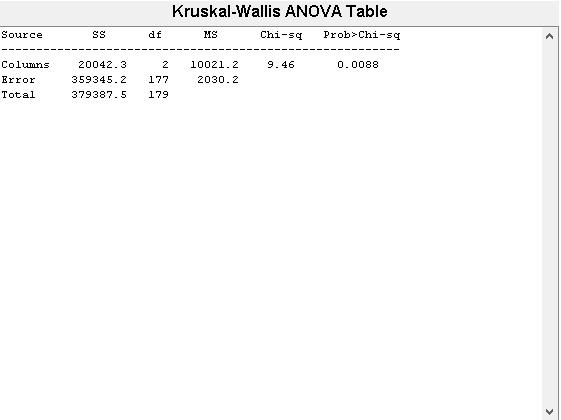
\includegraphics[width=0.7\textwidth]{images/Evaluation5.jpg}
    \caption{ANOVA table medium data}
    \label{fig:evaluation5}
\end{figure}

The P. value(Prob>Chi-sq) is 0.0088 and is below 0.05 similar to the above mentioned P value, where the Null hypothesis therefore also is rejected with the middle value test results.


% subsubsection middle_value_anova_table (end)

\subsubsection*{High Value ANOVA Table} % (fold)
\label{ssub:high_value_anova_table}

\begin{figure}[!htbp]
    \centering
    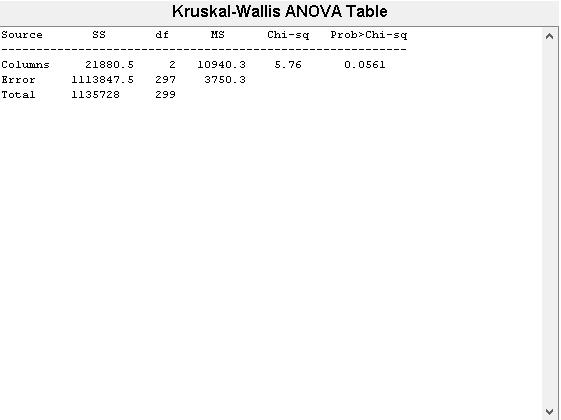
\includegraphics[width=0.7\textwidth]{images/Evaluation6.jpg}
    \caption{ANOVA table high data}
    \label{fig:evaluation6}
\end{figure}

The P. value(Prob>Chi-sq) is 0.0561 and is above 0.05 then indicates that we fail to reject the null hypothesis with specifically high value weather condition results.

There is no significant difference between the understanding of the non-speech auditory display of weather data using sonification techniques, compared to the understanding of visually presented weather information specifically for high value weather conditions.

Yet we cannot state that the samples are the same. Further elaboration will follow.

% subsubsection high_value_anova_table (end)

% subsection discussion (end)


\subsection{Kruskal-Wallis tests Boxplots} % (fold)
\label{sub:kruskal_wallis_tests_boxplots}

The low value boxplot (Figure~\ref{fig:evaluation3}) compliments the ANOVA table and illustrates significant difference of the independent variables between the visual, the sonification and both combined.
We can see that a large amount of participants answered correctly on the visual test, but a few. And with the sound and sound \& visual, the upper quartile indicates that from the median up to maximum, 50 \% of test participants answered incorrectly, as the correct answer was 1, being the label of low whereof a large amount of the test participants answered 2 or 3.  
This indicates that a large amount of the test participants misinterpreted the sonification of low weather conditions.

\begin{figure}[!htbp]
    \centering
    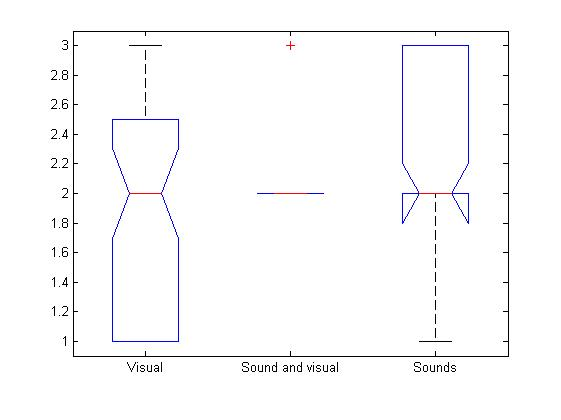
\includegraphics[width=.7\textwidth]{images/Evaluation7.jpg}
    \caption{Boxplot medium data}
    \label{fig:evaluation7}
\end{figure}

The middle value Boxplot (Figure~\ref{fig:evaluation7}) indicates a difference in the visual, sonification and sound \& sonification test results, which also has been defined as the alternative hypothesis has been accepted.

On all three groups, the median are 2, which is the correct label, middle value, and illustrates that a majority of the test participants answered correctly in each of the three tests.

The notched boxplot “Visual” illustrates that 50\% of the test participants answered 1, which is incorrect and lower than the intended formulation. There are however below 25\% who answered incorrectly in the test where Sound \& Visual was presented, and only 3 (high value) was answered as a wrong answer by a small number of the test participants.

Lastly the boxplot of sounds indicate that a majority answered correctly with 2, but 25\% answered 3, and another percentage of test subjects answered 1, which indicates that there are a majority of test subjects which misinterpreted the middle value sonifications. 

\begin{figure}[!htbp]
    \centering
    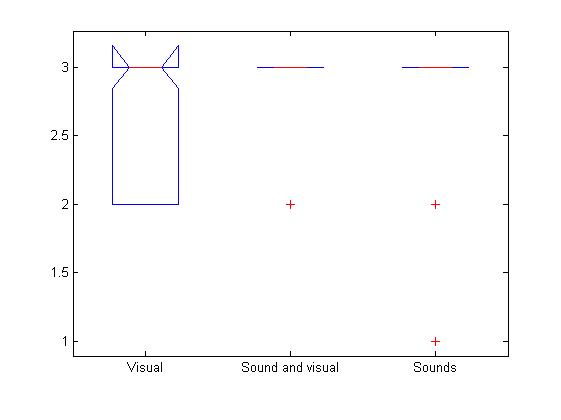
\includegraphics[width=.7\textwidth]{images/Evaluation8.jpg}
    \caption{Boxplot high data}
    \label{fig:evaluation8}
\end{figure}

The High-value boxplot of which the null hypothesis is accepted, there are no significant difference in the samples. 
They are however not similar.
The Visual sample indicates that 25\% of the test subjects thought of some or more of the visual interpretations of weather conditions as being a middle value.

There are however in the sound and visual sample below 25\% who thought that is was a medium value. 
And with the sound sample, below 25\% of the test participants thought that the sonification indicated either low or medium, leaving 75\% test participants answering correctly.

% subsection kruskal_wallis_tests_boxplots (end)

\FloatBarrier
\subsection{Pie charts} % (fold)
\label{sub:pie_charts}

Although the boxplot and ANOVA tables indicates any similarities or differences between the samples, they do not describe what specific sounds/visuals which had any impact or what could have been done differently or what specific sounds which were actually successful in conveyance of sonifications of weather data.
However, the following appendix(XX: Pie chart appendix)) indicates the percentage of correct responses of each weather category, and makes it possible for comparisons. 

% subsection pie_charts (end)

% section evaluation (end)